\documentclass[letterpaper]{article} 
\usepackage[left = 0.5in, right = 0.5in, top = 0.9in, bottom = 0.9in]{geometry}
\usepackage{enumitem}
\usepackage{multicol}
\usepackage[spanish]{babel}
\usepackage[utf8]{inputenc}
\usepackage{hyperref}
\usepackage{amsmath,amssymb,amsthm}
\usepackage{tikz-cd}
\usepackage{mathrsfs}
\usepackage[bbgreekl]{mathbbol}
\usepackage{dsfont}
\usepackage{graphicx}
\graphicspath{{img/}}

\newcommand{\op}{\operatorname}
\newcommand{\Op}{^{\op{op}}}
\newcommand{\scc}{\mathscr C}
\newcommand{\scd}{\mathscr D}
\newcommand{\sce}{\mathscr E}
\newcommand{\sci}{\mathscr I}
\newcommand{\scj}{\mathscr J}
\newcommand{\scx}{\mathscr X}
\newcommand{\var}{\mathrm{Var}}
\newcommand{\Id}{\operatorname{Id}}
\newcommand{\N}{\mathbb N}
\newcommand{\Z}{\mathbb Z}
\newcommand{\Q}{\mathbb{Q}}
\newcommand{\I}{\mathbb{I}}
\newcommand{\R}{\mathbb{R}}
\newcommand{\C}{\mathbb{C}}
\newcommand{\F}{\mathcal{F}}
\newcommand{\G}{\mathcal{G}}
\newcommand{\B}{\mathcal{B}}
\newcommand{\abs}[1]{\left\lvert #1 \right\rvert}
\newcommand{\inv}{^{-1}}
\renewcommand{\to}{\rightarrow}
\newcommand{\ent}{\Longrightarrow}
\newcommand{\E}{\mathbb{E}}
\renewcommand{\P}{\mathbb{P}}
\newcommand{\1}{\mathds{1}}
\renewcommand{\qedsymbol}{$\blacksquare$}

\theoremstyle{definition}
\newtheorem{dfn}{Definición}
\theoremstyle{definition}
\newtheorem{teo}{Teorema}
\theoremstyle{definition}
\newtheorem{cor}{Corolario}
\theoremstyle{definition}
\newtheorem{prop}{Proposición}
\theoremstyle{definition}
\newtheorem{obs}{Observación}


\title{\textbf{Cómputo Científico\\
Tarea 10\\
MCMC: Tarea final}}
\author{Iván Irving Rosas Domínguez}
\date{\today}

\DeclareSymbolFontAlphabet{\mathbbm}{bbold}
\DeclareSymbolFontAlphabet{\mathbb}{AMSb}
\DeclareMathSymbol\bbDelta  \mathord{bbold}{"01}

\begin{document}
\maketitle

%\begin{abstract}
%\end{abstract}

En ambos problemas hay que diseñar e implementar el MCMC, investigar sobre su convergencia 
y tener algún grado de certeza sobre si sí se está simulando de la posterior correspondiente.
Más aún, recuerde que se trata de un problema de inferencia: hay que hablar del problema en si,
comentar sobre las posteriores simuladas y posibles estimadores (a partir de la muestra de posterior)
que se pueden proporcionar de cada parámetro.
\begin{itemize}
    \item[\textbf{1.}]\textbf{(Problema en ecología)} Sean $X_1,...,X_m$ variables aleatorias 
    donde $X_i$ denota el número de individuos de una especie en cierta región. Suponga que 
    $X_i\big|N, \ p\sim$ Binomial$(N,p)$, entonces 
    \[
    f(\overline{x}|N,p)=\prod_{i=1}^{m}\frac{N!}{x_i!(N-x_i)!}p^{x_i}(1-p)^{N-x_i}.    
    \]
    Asumiendo la distribución a priori $p\sim$ Beta($\alpha,\beta)$ y $N\sim h(\cdot)$, donde
    $h$ es una distribución discreta en $\left\{0,1,2,...,N_{max}\right\}$, se tiene 
    definida la distribución posterior $f(N,P|\overline{x})$.

    A partir del algoritmo MH, simule valores de la distribución posterior usando un kernel híbrido.
    Para ello considere \textbf{como sugerencia} la siguiente distribución inicial para el MCMC
    \[
    p\sim \text{U}(0,1) \qquad \text{y} \qquad N\sim \text{U}_d\left\{\max_{i\in \{1,...,m\}}(x_i), \ \max_{i\in \left\{1,...,m\right\}}(X_i)+1,...,N_{max}\right\}    
    \]
    y las propuestas 
    \begin{itemize}
        \item[\underline{Propuesta 1:}] De la condicional total de $p$ (kernel Gibbs).
        \item[\underline{Propuesta 2:}] De la a priori.
        \item[\underline{Propuesta 3:}] Propuesta hipergeométrica (¿?).
        \item[\underline{Propuesta 4:}] Poisson: $N_p\sim \max_{i\in \{1,...,m\}}(x_i) +$ Poisson(?).
        \item[\underline{Propuesta 5:}] Caminata aleatoria
        \[
        N_p=N+\varepsilon, \qquad \P\left(\varepsilon=1\right)=\frac{1}{2}=\P\left(\varepsilon=-1\right).
        \]
    \end{itemize}
    Los datos son estos: 7,7,8,8,9,4,7,5,5,6,9,8,11,7,5,5,7,3,10,3.

    A priori, esperamos que sea difícil observar a los individuos entonces $\alpha=1,\beta=20$. La especie no 
    es muy abundante y entonces $N_{max}=1000$ y $h(N)=1/(N_{max}+1)$; $N\in \{0,1,2,...,N_{max}\}$.
    
    Las propuestas y distribución inicial para el MCMC de arriba son \textbf{solamente sugerencia}, propongan otras propuestas, 
    experimenten y comenten.\\

    \textbf{Solución:} se presenta el algoritmo solamente con la propuesta 2. El código relacionado a esta tarea se encuentra en el archivo $Computo tarea 9.py$.\\

    Para la solución de este ejercicio se implementa la semilla $seed=10$ para replicar resultados. Se crea un vector donde guardar los datos, y se crea
    la función $coc\_dist\_obj$, la cual toma los parámetros $N$ y $p$ tanto propuestos como actuales, así como los datos, y con base en todos ellos calcula el cociente 
    de Metrópolis-Hastings para implementar la propuesta 2. Es de destacar que, dado que la propuesta 2 consiste en justamente las distribuciones a priori de los parámetros 
    $N$ y $p$, se tiene entonces que al momento de hacer el cociente 
    \[
    \frac{f(Ny,py|\overline{x})q((Nx,px))|(Ny,py)}{f(Nx,px|\overline{x})q((Ny,py)|(Nx,qx))},    
    \]
    al ser la a posteriori proporcional a la verosimilitud multiplicado por la a priori de los parámetros,
    \[
        f(N,p|\overline{x})\propto f(\overline{x}|N,p)f(N,p)    
    \]
    la parte del cociente que tiene a las a priori, tanto como propuestas como la parte de la distribución a posteriori que es nuestra distribución objetivo, se cancela.
    Ello nos permite simplemente preocuparnos por el cociente de las expresiones 
    \[
        \prod_{i=1}^{m}\frac{N!}{x_i!(N-x_i)!}p^{x_i}(1-p)^{N-x_i}.
    \]
    tanto para $N,p$ propuestos y actuales. La expresión del cociente se encuentra en la 
    parte correspondiente a la función para la propuesta 2 del código del ejercicio. En ella se realizaron simplificaciones y manipulación de la expresión del cociente como la exponencial del 
    logaritmo de otras expresiones, lo cual es sumamente conveniente pues estamos tratando con factoriales y ello puede dar origen a errores numéricos. Asimismo, se realizan 
    algunos cambios de flotante a enteros y viceversa, con la finalidad de poder operar con cuidado los factoriales y los índices.
    \newline

    Es de destacar que, a pesar de las precauciones tomadas, los errores del estilo "overflow" se hacen presentes al correr el código, por lo que una implementación más 
    cautelosa de las expresiones sería ideal.
    \newline

    Una vez creada esta función, se crea la función que encarnará al algoritmo $MH\_gibbs$. Esta toma como argumentos tres parámetros: la cantidad de iteraciones, el 
    vector inicial y el vector de datos. Con la información del problema, se simula un vector de datos iniciales $m=(N,p)$, se imponen las condiciones $N_{max}=1000$, 
    $\alpha=1,\beta=20$ y $h$ se supone uniforme discreta en el conjunto $\{0,1,...,N_{max}\}$.\\

    Una vez hecho esto, se simula el vector inicial $(N,p)$ de acuerdo a lo pedido en el ejercicio y se ejecuta el algoritmo con $k=100_000$ iteraciones. Se obtiene la trayectoria 
    de la cadena, así como los histogramas de las variables tanto $N$ como $p$. Estos se presentan en las figuras 1, 2 y 3 respectivamente. Es de destacar que en los histogramas 
    de las variables se utiliza un burn-in de tamaño 1000. Lo anterior meramente con base en cuestiones empíricas y aprovechándonos del tamaño de muestra grande.
    
    \begin{figure}[h!]
        \centering
        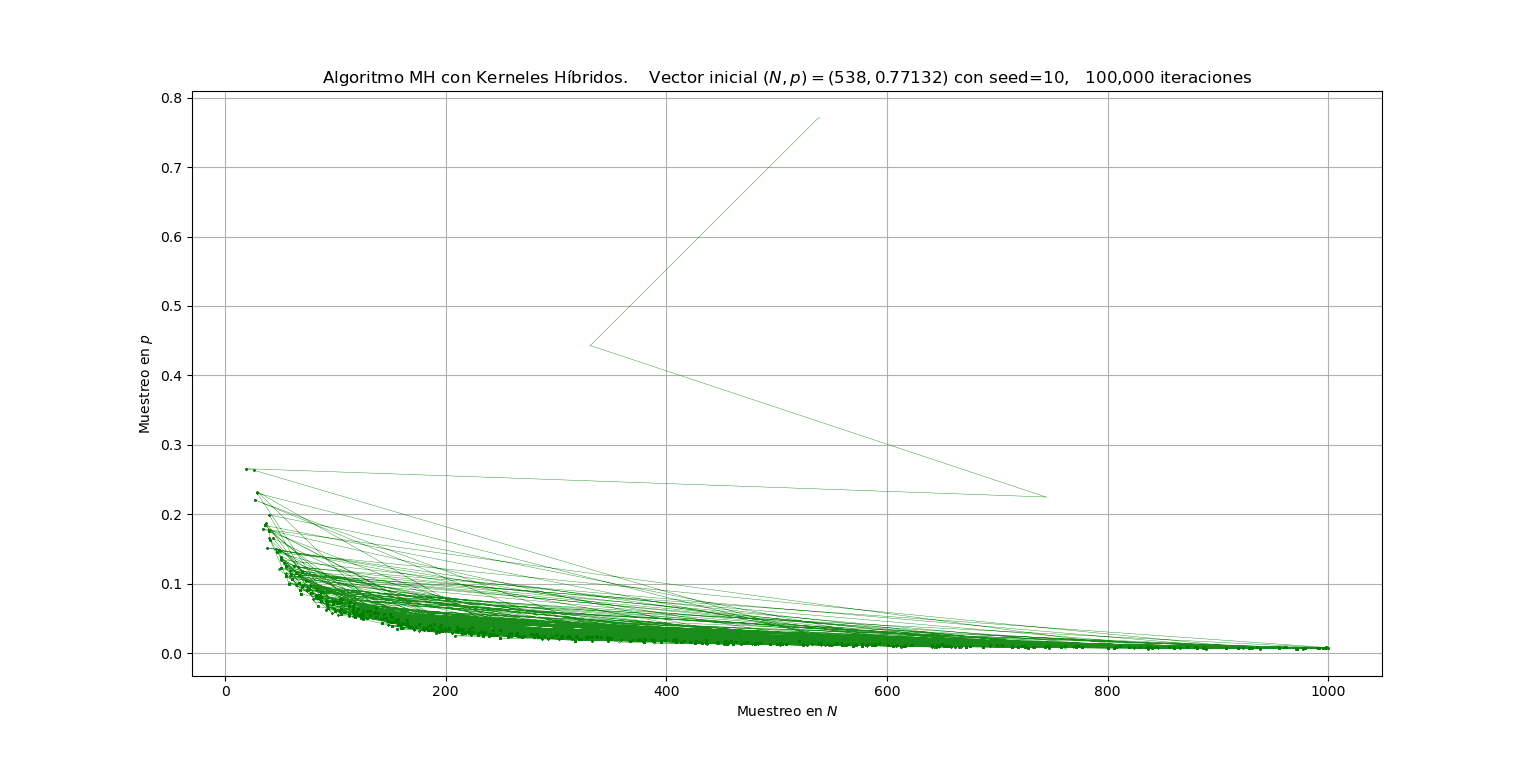
\includegraphics[width=\linewidth]{1.png}
        \caption{Gráfico del recorrido de la cadena.}
    \end{figure} 
    \begin{figure}[h!]
        \centering
        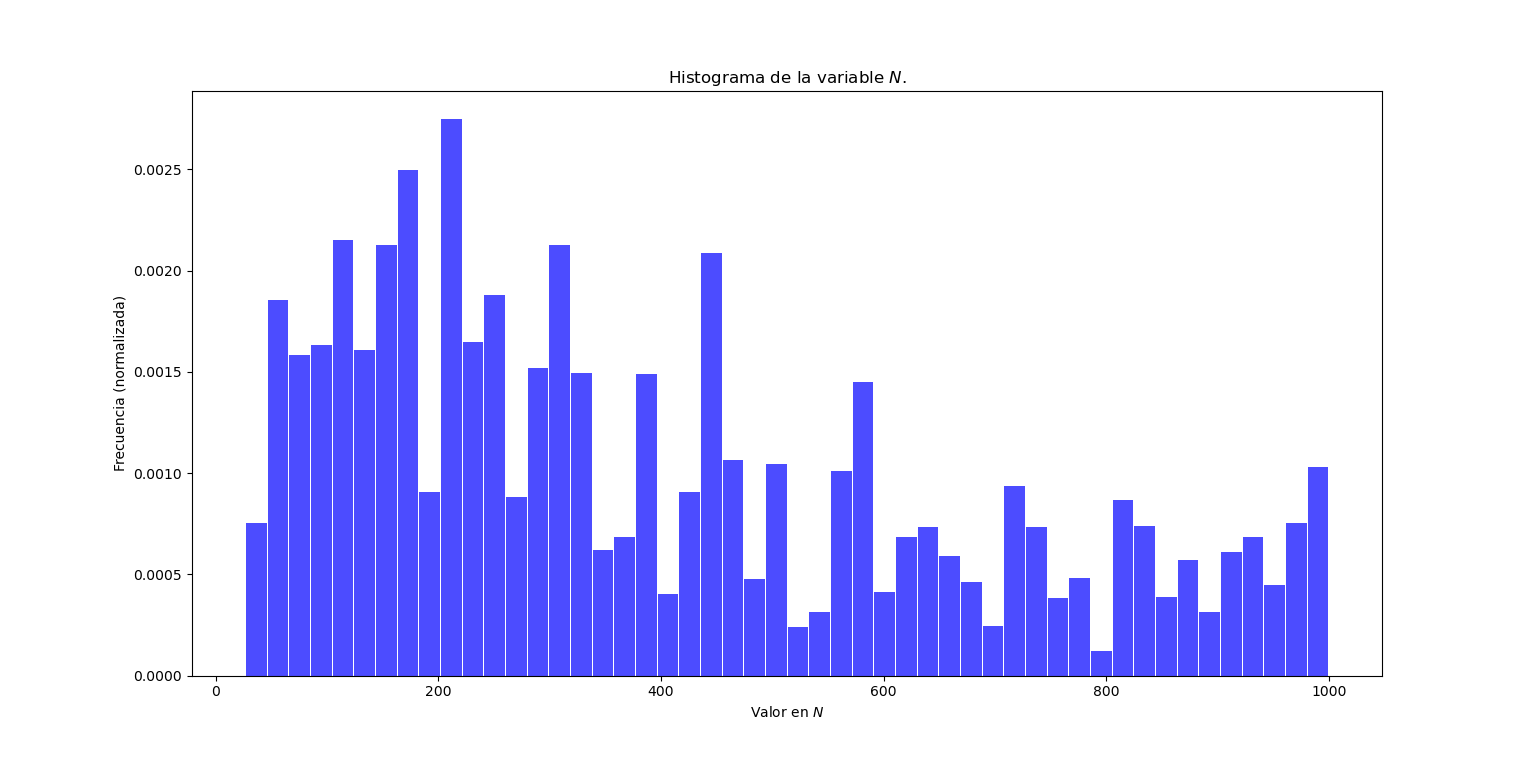
\includegraphics[width=\linewidth]{2.png}
        \caption{Histograma para $N$}
    \end{figure} 
    \begin{figure}[h!]
        \centering
        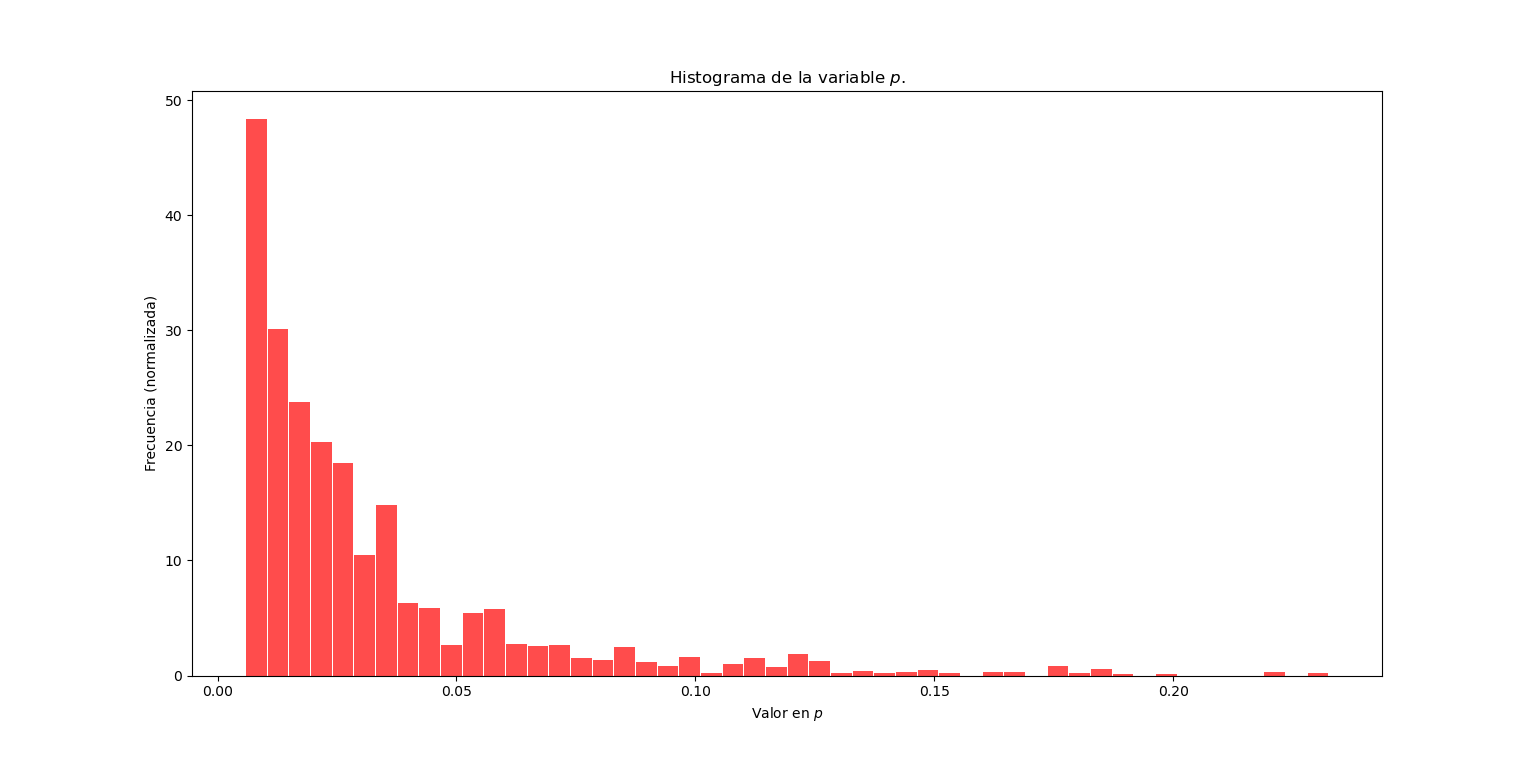
\includegraphics[width=\linewidth]{3.png}
        \caption{Histograma para $p$}
    \end{figure} 
    Observamos en la figura 1 la forma de una distribución no conocida. La misma se concentra alrededor de los valores entre 0 y 0.1 
    con respecto al parámetro $p$, mientras que con respecto al parámetro $N$, la mayor parte 
    de las muestras parecen ubicarse entre el 100 y el 800. Lo anterior se ve corroborado al extraer la 
    media de las muestras tanto en $N$ como en $p$, ya que los datos de la simulación nos 
    dicen que 396 es la media en $N$, y $0.0324$ es la media en $p$, lo cual está dentro 
    de lo que pudimos observar meramente de la gráfica.
    \newline

    Los histogramas en $N$ muestran un comportamiento atípico, el cual no es reconocible 
    en comparación con distribuciones continuas conocidas.\\

    No obstante los histogramas en $p$ muestran un comportamiento similar al exponencial, aunque con 
    valores atípicos y pesados en la cola derecha. Esto podría ser indicador de que la distribución de $p$ 
    sigue una distribución de colas pesadas.
    \newline

    Un estudio más a profundidad del contexto de esta distribución bien puede arrojar 
    luz sobre si los resultados obtenidos son deseables o pobres.

    \item[\textbf{3.}] Investiga y describe muy brevemente los softwares OpenBugs, Nimble, JAGS, DRAM, Rtwalk, Mcee Hammer, PyMCMC.
    Hacemos un breve recuento de cada uno de los 7 softwares anteriores:
    \begin{enumerate}
        \item[\textbf{OpenBugs}] Es un software de código abierto para modelación Bayesiana. Desarrollado a partir de WinBUGS (proyecto desarrollado en el MRC Biostatistics de la universidad de Cambridge y 
        el Imperial College School of Medicine en 1997) actualmente no está continuado en su desarrollo, pero la versión actual y las versiones anteriores están disponibles en la página del software:
        \url{https://www.mrc-bsu.cam.ac.uk/software/bugs/openbugs/}. Tanto este software como sus antecesores están basados en el proyecto BUGS (Bayesian inference Using Gibbs Sampling), 
        proyecto a su vez comenzado en 1989.
        \newline

        De acuerdo al sitio web anterior, OpenBUGS provee un mayor espectro funcional que su software predecesor WinBUGS en cuanto 
        al muestreo utilizando MCMC, además de correr de manera nativa en Linux. Asimismo, desarrollos futuros con base en el 
        proyecto BUGS se enfocan actualmente en MultiBUGS, el cual es un software que utiliza a OpenBUGS pero que 
        tiene una mejora en cuanto al tiempo de ejecución.

        \item[\textbf{Nimble}] De las siglas Numerical Inference for statistical Models using Bayesian and Likelihood Estimation, 
        es un sistema para construir y compartir métodos de análisis para 
        modelos estadísticos, específicamente para modelos jerárquicos y métodos computacionalmente intensivos.
        \newline

        El software está construido en R, pero para compilar los modelos y algoritmos que 
        el usuario cree en él utiliza C++ para ganar velocidad. Esencialmente Nimble posee tres componentes:
        \begin{itemize}
            \item Un sistema para utilizar modelos escritos en el modelo de lenguaje de BUGS como 
            objetos programables en R.
            \item Una librería inicial de algoritmos para modelos escritos en BUGS, incluyendo MCMC básico.
            \item Un lenguaje inmerso en R para programar algoritmos para modelos, ambos compilados a través 
            de código en C++ y cargados en R.
        \end{itemize}
        Su página, en constante actualización, es \url{https://r-nimble.org/}

        \item[\textbf{JAGS}] De las siglas Just Another Gibbs Sampler, es un programa para análisis de modelos Bayesianos jerárquicos
        que utiliza simulación por MCMC. De acuerdo a su página principal, JAGS fue escrito con tres motivos en mente:
        \begin{itemize}
            \item Tener una multiplataforma como motor del lenguaje BUGS
            \item Ser un software con posbilidad de extensiones, permitiendo a usuarios escribir sus propias funciones, distribuciones y samplers.
            \item Ser una plataforma para experimentación con ideas en modelación Bayesiana.
        \end{itemize}
        JAGS es prácticamente libre. Se puede modificar y redistribuír bajo ciertas condiciones. Su página 
        oficial sigue la siguiente liga: \url{https://mcmc-jags.sourceforge.io/}

        \item[\textbf{DRAM}] DRAM son las siglas de Delayed Rejection Adaptive Montecarlo. Es un método que utiliza tanto Montecarlo Adaptativo como Delayed  
        en pro de mejorar la eficiencia del algoritmo Metrópolis-Hastings. El Montecarlo adaptativo es una variante de MCMC en el cual el algoritmo va 
        ajustándose de acuerdo a la trayectoria que ha tenido el proceso, a costa de perder la propiedad de Markov, aunque preservando las propiedades 
        ergódicas de la cadena. El método de Delayed Rejection consiste en que, en el momento en que una propuesta es rechazada, en lugar de avanzar el tiempo y quedarnos en el 
        mismo estado, se lanza otra propuesta. La idea es que se retarde el rechazo (delay the rejection), y las probabilidades de aceptar la segunda propuesta se 
        calculan de tal manera que se preserve la reversibilidad de la cadena. este método puede ser adaptado para varias propuestas de rechazo. A diferencia de MCMC adaptativo, 
        con esta técnica de retraso al rechazar se preserva la propiedad de Markov de la cadena.\\

        DRAM tiene varias maneras de implementarse dependiendo del uso de ambas estrategias anteriores. Generalmente, luego de que una primera propuesta es rechazada, 
        se utiliza el Delayed Rejection proponiendo un nuevo estado para la cadena con base en la historia de la cadena, usando la idea de Adaptive Montecarlo.\\

        Un software que implementa esta idea es MatDRAM, una librería de Mathlab. MatDRAM es parte de la librería ParaMonte, especializada en simulación Monte Carlo.
        \item[\textbf{Rtwalk}] La implementación en R del algoritmo 't-walk' MCMC, un sampleador para distribuciones continuas arbitrarias de propósito general.
        \item[\textbf{Mcee Hammer}] Es una implementación bajo licencia del MIT del Affine Invariant Markov chain Monte Carlo Ensemble sampler (emcee), propuesto 
        por Goodman \& Weare en 2010. Se trata de una familia de métodos MCMC cuyo rendimiento no se 
        ve afectado por transformaciones afines del espacio. Tales algoritmos, de acuerdo al abstract 
        del artículo presentado por los autores, son fáciles de construir y requieren poco o nulo esfuerzo computacional extra.
        Se asegura que deberían ser particularmente útiles para muestrear distribuciones mal escaladas. Asimismo,
        pruebas computacionales muestran que estos métodos invariantes bajo transformaciones afines 
        pueden mejorar la velocidad significativamente comparado con los métodos MCMC estándar cuando
        se tratan de distribuciones altamente asimétricas (un alto valor de skewness).
        \item[\textbf{PyMCMC}] Es descrito como un paquete de Python que ayuda en la construcción de samplers tipo MCMC, y ayuda a reducir la
        posibilidad de cometer un error de código, aí como la minimización de código repetitivo. Este software contiene clases para Gibbs, MH, MH independiente, RWMH,
        entre otros. Es sencillo de optimizar, tomando ventaja de las librerias de Python Numpy y Scipy, así como fácilmente extendible con C o Fortran. 
    \end{enumerate}
\end{itemize}
\end{document}